\documentclass{article}

\usepackage{graphicx}
\usepackage{tikz}
\usepackage{tikzsymbols}
\usetikzlibrary{calc,patterns,shapes.geometric}
\pagestyle{empty}
\usepackage[margin=0pt]{geometry}
\geometry{papersize={14in,12in}}

\def\centerarc[#1](#2)(#3:#4:#5){\draw[#1] ($(#2)+({#5*cos(#3)},{#5*sin(#3)})$) arc (#3:#4:#5);}

\begin{document}
	\begin{figure}
		\centering
		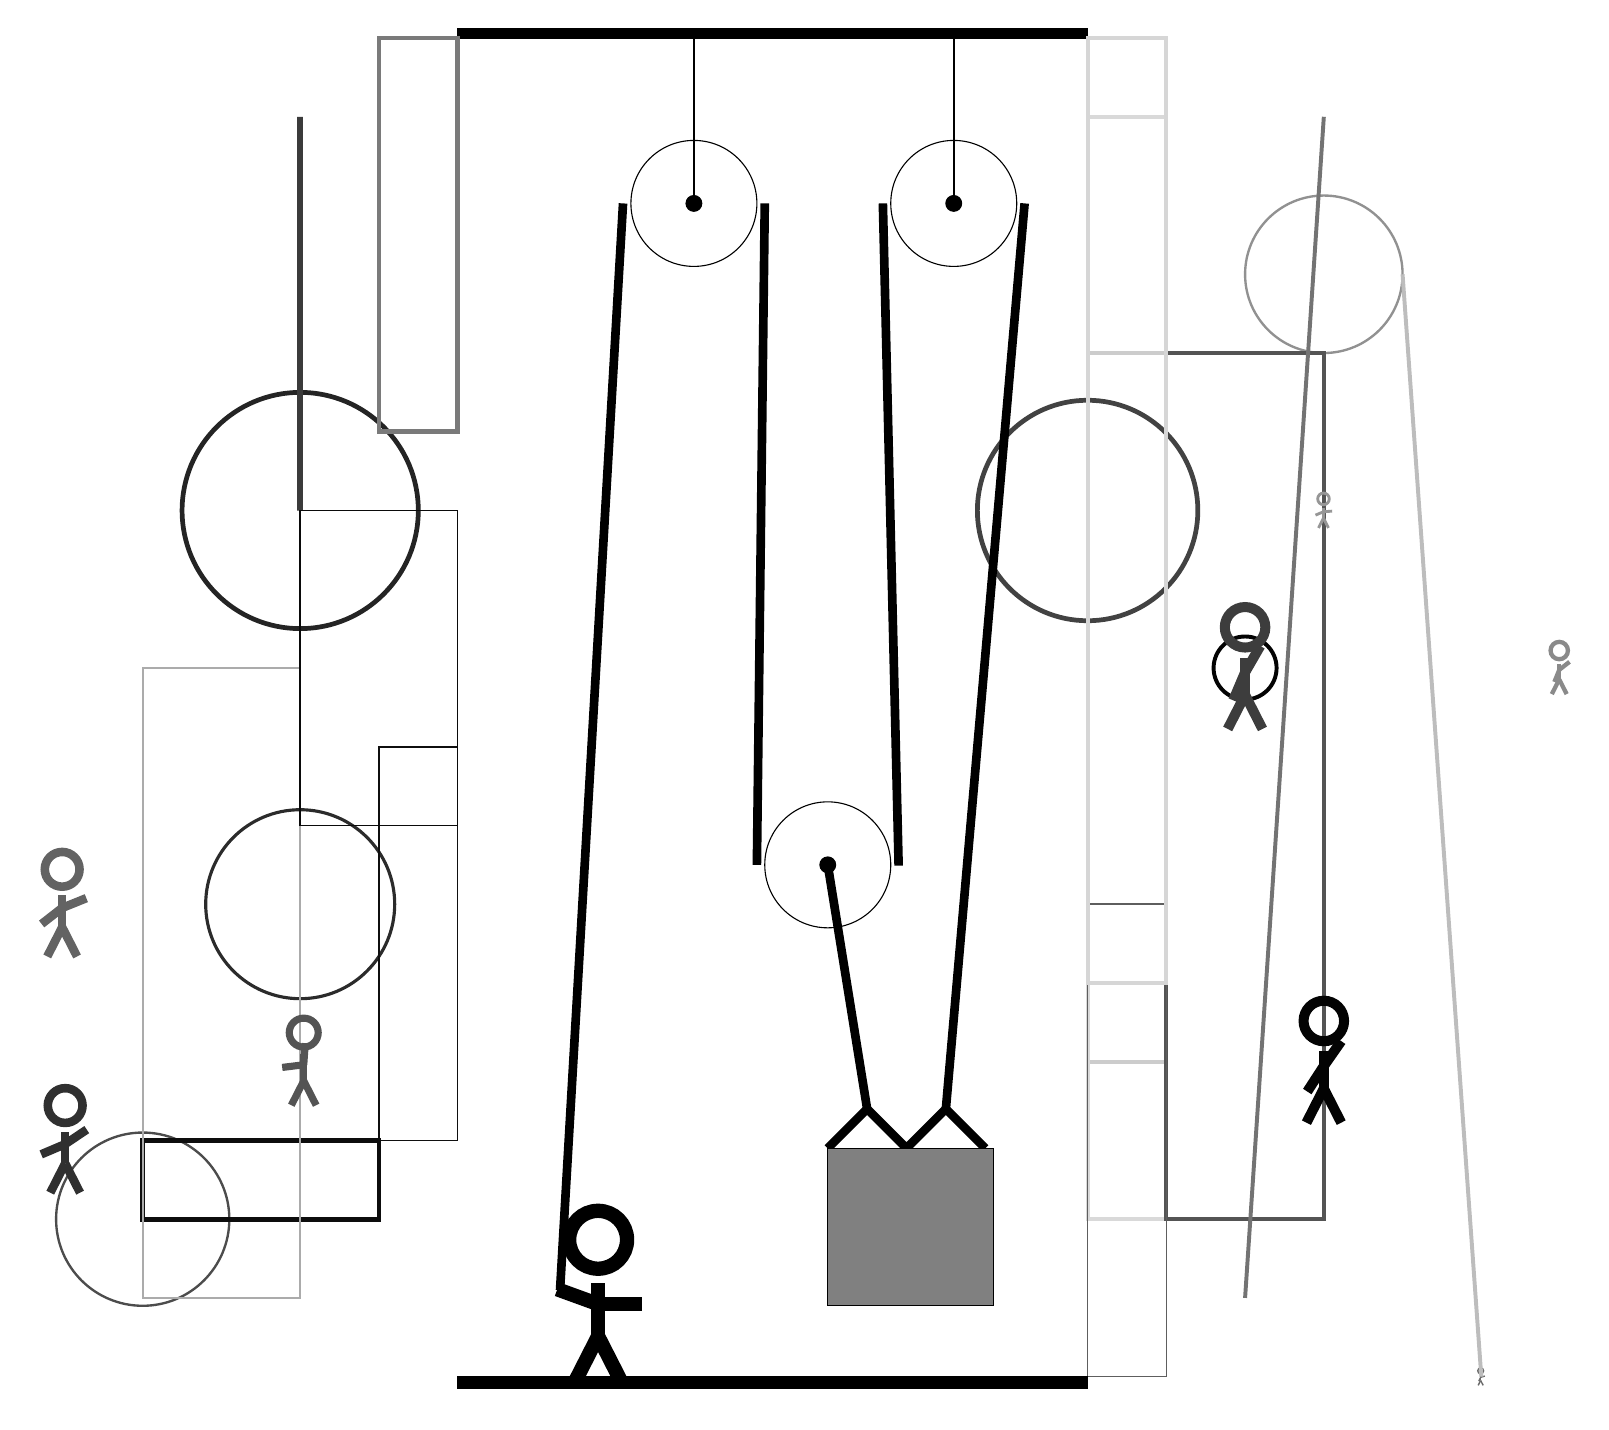
\begin{tikzpicture}
			%%%%% START %%%%%
			
			\draw[fill=black] (-2, 14) rectangle (6, 14.125);
			
			\draw (1, 11.9) circle (0.8);
			\draw[fill=black] (1, 11.9) circle (0.1);
			\draw[thick] (1, 11.9) -- (1, 14);
			
			\draw[line width=0.5mm, color=black!20] (7, 10) rectangle (6, 1);
			
			\draw [line width=0.3mm, color=black!70](-6, -1) circle (1.1);
			\draw [line width=0.6mm, color=black!86](-4, 8) circle (1.5);
			\draw [line width=0.3mm, color=black!43](9, 11) circle (1.0);
			\draw[line width=0.5mm, color=black!15] (6, -1) rectangle (7, 13);
			\draw[line width=0.5mm, color=black!67] (7, -1) rectangle (9, 10);
			
			\draw[line width=0.6mm, color=black!95] (-3, 0) rectangle (-6, -1);
			\node[line width=0.5mm, color=black!99] at (9, 1) {\Strichmaxerl[7][57][55]};
			\node[line width=0.2mm, color=black!61] at (-7, 3) {\Strichmaxerl[6][38][22]};
			
			\draw [line width=0.4mm, color=black!83](-4, 3) circle (1.2);
			\draw[line width=0.2mm, color=black!63] (7, -3) rectangle (6, 3);
			\draw [line width=0.6mm, color=black!74](6, 8) circle (1.4);
			\node[line width=0.6mm, color=black!58] at (11, -3) {\Strichmaxerl[1][65][16]};
			
			\draw[line width=0.3mm, color=black!33] (-4, -2) rectangle (-6, 6);
			\draw[line width=0.5mm, color=black!55](8, -2) -- (9, 13);
			\draw [line width=0.5mm, color=black!99](8, 6) circle (0.4);
			\draw[line width=0.7mm, color=black!77] (-4, 13) rectangle (-4, 8);
			\draw[line width=0.2mm, color=black!94] (-3, 5) rectangle (-2, 0);
			\node[line width=0.2mm, color=black!41] at (9, 8) {\Strichmaxerl[2][23][4]};
			
			\node[line width=0.2mm, color=black!67] at (-4, 1) {\Strichmaxerl[5][7][86]};
			\draw[line width=0.6mm, color=black!52] (-3, 9) rectangle (-2, 14);
			\draw[line width=0.5mm, color=black!26](11, -3) -- (10, 11);
			\node[line width=0.6mm, color=black!46] at (12, 6) {\Strichmaxerl[3][68][38]};
			\draw[line width=0.5mm, color=black!16] (7, 2) rectangle (6, 14);
			\node[line width=0.2mm, color=black!81] at (-7, 0) {\Strichmaxerl[6][23][34]};
			
			\draw[line width=0.2mm, color=black!96] (-4, 4) rectangle (-2, 8);
			
			\node[line width=0.7mm, color=black!76] at (8, 6) {\Strichmaxerl[7][67][60]};
			
			\draw (4.3, 11.9) circle (0.8);
			\draw[fill=black] (4.3, 11.9) circle (0.1);
			\draw[thick] (4.3, 11.9) -- (4.3, 14);
			
			\draw (2.7, 3.5) circle (0.8);
			\draw[fill=black] (2.7, 3.5) circle (0.1);
			
			\draw[line width=1.1mm]  (2.7, -0.1) -- (3.2, 0.4) -- (3.7, -0.1) -- (4.2, 0.4) -- (4.7, -0.1);
			\draw[fill=black!50] (2.7, -0.1) rectangle (4.8, -2.1);
			
			\draw[line width=1.1mm](-0.7, -1.9) -- (0.1, 11.9);
			\centerarc[line width=1.1mm](1, 11.9)(0:180:0.9);
			\draw[line width=1.1mm](1.9, 11.9) -- (1.8, 3.5);
			\centerarc[line width=1.1mm](2.7, 3.5)(180:370:0.9);
			\draw[line width=1.1mm] (3.6, 3.49) -- (3.4, 11.9);
			\centerarc[line width=1.1mm](4.3, 11.9)(0:180:0.9);
			\draw[line width=1.1mm](4.2, 0.4) -- (5.2, 11.9);
			\draw[line width=1.1mm] (3.2, 0.4) -- (2.7, 3.5);
			
			\node at (-0.2, -2) {\Strichmaxerl[10][-20][0]};
			
			\draw[fill=black] (-2, -3) rectangle (6, -3.15);
			
			%%%%% END %%%%%
		\end{tikzpicture}
	\end{figure}	
\end{document}